\subsection{Thread switching in Unix}
Thread switching is the process of interrupting the execution of the CPU to store its current work and load other work. When this work is in the same virtual memory space, this is known as a thread rather than a process. This mechanic can allow Operating Systems to provide more advanced features such as perceived multitasking and interrupt based input handling. In Unix, context switching is performed by saving the current process to the Process Control Block (PCB) before loading the new process from the PCB. The PCB contains all of the data relevant to each processes including the registers, stack pointers, program counter and page tables. This switching can have a significant impact on performance as caches relevant to the previous thread must be flushed as they all reference a previous thread so cache hits reduce dramatically. Allowing this context switching means that each thread can operate within a time-slice dictated by the scheduler. Each thread will be given a certain amount of time to get is work done, before it is forced to wait for other processes.

The context switch is only half of the problem with thread switching. The other half is choosing which thread to run after a switch. This problem can be solved in many different ways, and each solution is better suited for different needs. These solutions are known as policies. Policies which exist include:

\begin{itemize}
	\item Round Robin (RR)
		  This policy will run each thread in turn for a specific time-slice. It is one of the fairest easiest algorithms
	\item First In First Out (FIFO)
	 	  This policy will run each thread to completion before moving to a new thread. 
	\item Shortest Job First (SJF)
		  This policy will run the shortest job to completion before moving on to the next shortest job. This results in lower average waiting times, but can also result in time starvation for longer jobs. This is where the longer jobs don't get any time to execute as there are always shorter job available. 
\end{itemize}


\subsection{The challenges of thread switching}
\label{chap:Threading}
That challenges of thread switching in ARM stem from the difficulty in storing a threads context in a way which is recoverable from any point without losing any state. Each thread must save its own registers, stacks, program counter, processor flags and link register. A good place to tackle this problem is to start from looking at how a procedure call works in ARM. Procedure calls in ARM are somewhat similar in concept, but they differ in scope. The procedure calls \cite{arm_man} I used in ARM consisted of the following steps
\begin{itemize}
	\item Move the LR onto the stack 
	\item Push non-parameter registers
	\item Execute the required procedure
	\item Update the defined output registers
	\item Recover the non-parameter registers from the stack
	\item Pop the LR back
	\item Return to the call location
\end{itemize} % Might be good to compare my procedure calls to the arm standard
This structure for a procedure call allows me to nest procedure calls within each other where necessary. Where the thread switching protocols differ is that they can't merely push registers to the stack. This is because, for each thread running, no thread should have to concerned with the others' existence. Each thread should be able to access the resources available without any concern that the other threads could be modifying the contents of the stack or a threads registers. In a sense threads should be invisible to each other. This raises several issues:
\begin{itemize}
	\item When should I run the context saving procedure to perform the time slicing?
	\item When can I safely interrupt?
	\item How do you keep the user's stack consistent for each thread?
	\item How do you store and load a threads' context without corrupting the registers or CPSR?
\end{itemize}
\subsubsection{When is the time-slicing procedure called?}
This is the easiest of the challenges above to solve. One of the plug-ins provided in the installation for Komodo is a configurable timer which can cause an interrupt. This is a natural entry point for the time slicing procedure, as a successfully implemented interrupt should be handled invisibly relative to the currently executing program. This is essentially what I want to occur. The executing program halts for the interrupt, which then gives control to another program, until another time slice is complete and control is returned to the original program. Of course in this example I am using two threads, but it can generalise to more threads. 
\begin{figure}[ht!]
	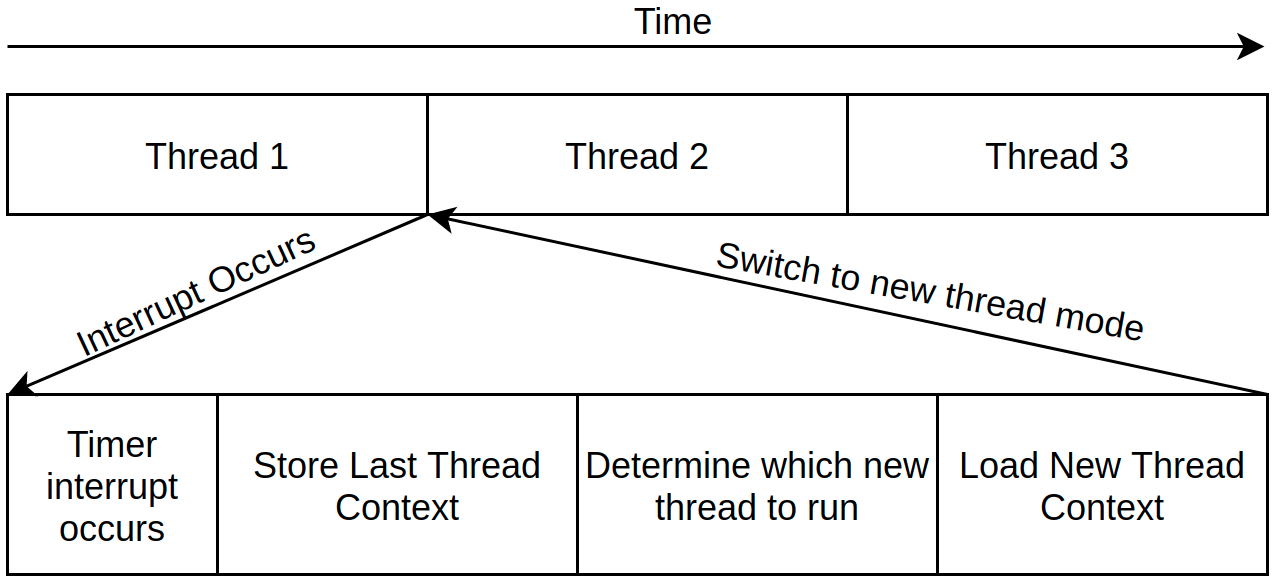
\includegraphics[width=\linewidth]{figures/cswitch.png}
	\caption{Context switching procedure for my system}
	\label{fig:cswitch}
\end{figure} 
\subsubsection{When can I safely interrupt?}
This is the next easiest challenge to solve. While it is possible to implement complex behaviours in ARM such as nested interrupts without extra hardware support, the software complexities required to implement it are usually not worth the benefits. To implement nested interrupts properly, additional hardware is needed. Allowing nested interrupts can make it very convoluted (but not impossible) to return the processor state to its precise state before any interrupts had occurred. The only upside of this added complexity is that you can reduce the latency in which you handle interrupts, which I could see being useful in some situations (such as a real-time system) but not in this one. Therefore, the solution is to leave interrupts as disabled during a standard interrupt call. Similarly, I would disable interrupts during a supervisor call, as it would simplify saving the state of the processor as I don't need to ensure the consistency of the supervisor stack.
\subsubsection{How do I ensure the user stacks consistency?}
The solution to this problem looks more simple than it is to implement. During thread creation, I assign each thread its own user stack to ensure that each program can operate on its own stack independently. The memory space assigned to each thread is statically assigned on start up according to a constant MAX\_THREADS. This constant defines the maximum number of threads which I allow, and allocates memory accordingly and divides it amongst the threads.  Once I have created this memory space, when I give a call to create a new thread, I can pick the first free stack space in my process control block and calculate a stack pointer for it. The reset procedure also has to account for this set-up as the main thread has to be treated in same way as any other thread.  This means that on reset, the correct data must be inserted into my process control block to mimic a call to my thread creation procedure. Now that each thread has its own stack pointer, saving a thread's stack during a context switch is as simple as saving my stack pointer.
\newpage
\subsubsection{How do you store and load a thread's context?}


\begin{wrapfigure}{l}{0.6\textwidth}\centering
	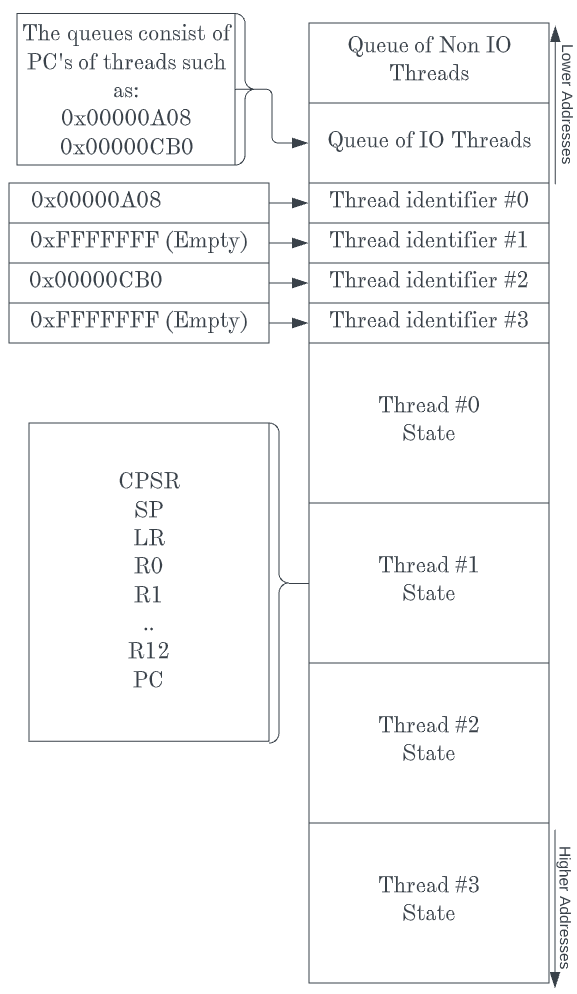
\includegraphics[scale=0.335]{figures/PCB.png}
	\caption{The memory layout of the PCB.}
	\label{fig:PCB}
\end{wrapfigure} 
This is the hardest problem I encountered when implementing threading. The loading and storing of a thread's context requires me have an organised way of storing and recovering each processor state. This is when the PCB comes in. This stores all the essential data neccesseary to restore a threads state. The PCB consists of the setup as seen in  Figure \ref{fig:PCB}. The PCB holds the state of saved threads at any given point. A thread's state is represented by first storing its PC in either the IO thread queue or the Non IO thread queue, depending on whether it was created with access to the virtual keyboard.
Once a thread is pushed onto a queue, its PC is used as an identifier in the thread identifier block. This block is an array, in which a thread is inserted at the first free location as designated by a -1 (0xFFFFFFFF). The index of the thread's PC then acts as an index for the thread states. The thread state at that index will then hold the registers for the thread. The registers are stored in the order shown on the left with the CPSR, SP and LR being stored before R0 - R12 and then the PC. An option I had to consider when creating this memory structure was how I was going to identify my threads. Most modern computers use a unique process identifier (PID) to reference a thread or process. %Probably a good point for a reference about operating systems
I briefly considered implementing this rather than identifying threads via their program counter however I felt that PIDs are more useful for a processor where a process might be executed on an arbitrary core rather than a single core. In my system, as there is only one `core` nothing can change the PC without running the code, so it acts as a decent primary key. This system does come with some caveats which I address in the evaluation in section \ref{threadingeval}.

The order of the registers is specific to aid the context switching procedure, specifically the loading of the previous state. To perform the load, first the scheduler has to determine which thread to revive, and then get a pointer to the CPSR in the thread state. Once it has this pointer and has taken the thread identifier off of the queue and the thread identifier block it can perform the load in four simple instructions.

\begin{lstlisting}[
	style = myListingStyle,
	caption = {Return Procedure.}
	]
	;R3 Points to the start of the thread state to be loaded.
	LDMIA R3!, {R4}
	MSR SPSR, R4
	LDMIA R3!, {SP, LR}^
	LDMIA R3, {R0 - R12, PC}^
\end{lstlisting}

These instructions work by manipulating the address in R3 which points to the CPSR. The first instruction loads the CPSR into R4, and writes back the increased address to R3. The second instruction updates the SPSR, so that when the mode is switched the thread's CPSR gets updated correctly. The third instruction copies the SP and LR into the user's SP and LR and then writes back the incremented address. The final instruction loads the thread's registers including the PC and causes the SPSR to be copied into the CPSR.

The procedure to store threads is somewhat more convoluted than the loading procedure. Once the address of the threads state is calculated, the first task is store the thread's CPSR. This is done by storing the current SPSR, as this procedure is called from IRQ mode so the SPSR holds a copy of the last thread's CPSR. Then to store the SP and LR, I use the \verb|STMIA| commands with the caret. This allows me to access the user mode registers. This is important as different modes have their own copies of the SP and LR which the caret enables me to access. I enter this procedure from my IRQ handler, which will push my user register to the stack as its first action. I have to retrieve these registers first by popping them. Once popped I then need to store them to the PCB via pushing. I then have to reset the SP to before the register R0 - R12 are pushed. This is  to ensure that the SP is correct for the next time that IRQ mode is entered. If this step is not taken, then every time the time slicing operation is called, the IRQ stack will grow by thirteen bytes. This will then cause the stack to overrun, which is unrecoverable, at least in this system.


\subsection{Integration with the virtual keyboard}
A part of the reason to implement threading was to enable efficient querying of the keyboard via interrupts enabling halted IO threads. Due to this it was important to ensure that the virtual keyboard could seamlessly integrate with the threading system. On account of this I developed a second method to query my keyboard as an alternative to my polling method. This method is composed of the following steps:

\begin{itemize}
	\item The thread makes a call to SVC\_11 to halt the thread
	\item The system saves the halted thread
	\item The system switches to another thread
	\item The keyboard throws an interrupt on input
	\item The system context switches back to initial halted thread
	\item The keyboard is queried.
\end{itemize}
This method uses the same method to query the keyboard as my polling method, but it differs in that it only needs to check the keyboard once as it will wait until the keyboard alerts it to new data. 

\subsection{Sheduling}
The scheduler is the piece of software which assigns resources to perform tasks. In my OS this equates to assigning CPU time, however it other systems these resources could be other things such as giving a process access to lower latency execution. This is most useful for real-time processes. Linux uses an algorithm called Completely Fair Scheduling (CFS) \cite{CFS}. This algorithm is similar to a round robin algorithm, with the key difference that the time slices are dynamic according to how many processes are currently running. For example if there are currently N processes in the system will allocate a time slice of time\_slice = scheduler\_latency/N. To actual determine which process will be run next, the scheduler maintains a running total of the execution time for each process. To determine the next process to run, the process with the lowest total execution time is chosen. 
My scheduler implements a far simpler form of this. My scheduler is primarily based off of a First-In-First-Out (FIFO) list. This is as the name implies. Threads are appended to the back of the queue, and the thread a the front of the queue is popped off. The difference with my implementation from a usual FIFO policy is that IO threads have the highest priority. When an interrupt is received from the keyboard, to reduce latency, the context switch saving operation is run and the oldest IO thread is loaded. This enables this IO thread to access the keyboard data as soon as the data is available. While this is not necessarily fair to other processes, it is balanced by the fact that the IO thread will most likely be halted for a while whilst waiting for IO to trigger an interrupt. 

\subsection{Evaluation of threading system}
\label{threadingeval}
The threading system implemented here work well aside from a few issues which need resolving. Firstly, my implementation of the PC as a thread identifier was a mistake as it means that the PCB can be read incorrectly if two threads operate on the same code. If two threads become saved in the PCB with the same PC then there is the potential for trouble to occur. When time slicing, the PCB is read by popping the new thread PC from the queue. It then runs a find operation on the block of thread identifiers to find the first occurrence of the PC in the block. The index of this data is used to determine which thread state is loaded. Due to the fact that it will only find the first occurrence of the PC, it will still load a thread correctly. This thread will then run resulting the PC changing, so when the program is time sliced out again, the conflict will resolve itself. The issues will only occur when the thread\_end function is called and two stored threads have the same PC. In this event if the thread\_end function is called on one of these conflicting identifiers, the wrong thread might get killed. This is unlikely to occur, but not impossible, in addition the likelihood of this occurring would go up as more threads are introduced. While unlikely, this should really be resolved as if it were to occur in a live system, finding this as the cause would be difficult to track down, as it would only occur intermittently. Issues like this are harder to reproduce, and therefore harder to track down. In future I would implement a PID system, much like unix provides. This system would name and reference threads via a unique ID allocated sequentially according to the order of process creation. This would resolve the conflicting identifier issue.
















